
\documentclass[conference]{IEEEtran}

\usepackage[pdftex]{graphicx}
\graphicspath{ {../images/} }
\usepackage{caption}
\usepackage{subcaption}
\usepackage{float}
\usepackage{amsmath}

\usepackage{hyperref}
\hypersetup
{
    colorlinks=true,
    linkcolor=black,   
    urlcolor=blue,
    citecolor=black,
}

\usepackage{pdfpages}
\renewcommand{\familydefault}{\sfdefault}

% *** ALIGNMENT PACKAGES ***
%
%\usepackage{array}
% Frank Mittelbach's and David Carlisle's array.sty patches and improves
% the standard LaTeX2e array and tabular environments to provide better
% appearance and additional user controls. As the default LaTeX2e table
% generation code is lacking to the point of almost being broken with
% respect to the quality of the end results, all users are strongly
% advised to use an enhanced (at the very least that provided by array.sty)
% set of table tools. array.sty is already installed on most systems. The
% latest version and documentation can be obtained at:
% http://www.ctan.org/tex-archive/macros/latex/required/tools/


%\usepackage{mdwmath}
%\usepackage{mdwtab}
% Also highly recommended is Mark Wooding's extremely powerful MDW tools,
% especially mdwmath.sty and mdwtab.sty which are used to format equations
% and tables, respectively. The MDWtools set is already installed on most
% LaTeX systems. The lastest version and documentation is available at:
% http://www.ctan.org/tex-archive/macros/latex/contrib/mdwtools/


% IEEEtran contains the IEEEeqnarray family of commands that can be used to
% generate multiline equations as well as matrices, tables, etc., of high
% quality.


% *** SUBFIGURE PACKAGES ***
%\usepackage[tight,footnotesize]{subfigure}
% subfigure.sty was written by Steven Douglas Cochran. This package makes it
% easy to put subfigures in your figures. e.g., "Figure 1a and 1b". For IEEE
% work, it is a good idea to load it with the tight package option to reduce
% the amount of white space around the subfigures. subfigure.sty is already
% installed on most LaTeX systems. The latest version and documentation can
% be obtained at:
% http://www.ctan.org/tex-archive/obsolete/macros/latex/contrib/subfigure/
% subfigure.sty has been superceeded by subfig.sty.


% *** FLOAT PACKAGES ***
%
%\usepackage{fixltx2e}
% fixltx2e, the successor to the earlier fix2col.sty, was written by
% Frank Mittelbach and David Carlisle. This package corrects a few problems
% in the LaTeX2e kernel, the most notable of which is that in current
% LaTeX2e releases, the ordering of single and double column floats is not
% guaranteed to be preserved. Thus, an unpatched LaTeX2e can allow a
% single column figure to be placed prior to an earlier double column
% figure. The latest version and documentation can be found at:
% http://www.ctan.org/tex-archive/macros/latex/base/



\usepackage{stfloats}
% stfloats.sty was written by Sigitas Tolusis. This package gives LaTeX2e
% the ability to do double column floats at the bottom of the page as well
% as the top. (e.g., "\begin{figure*}[!b]" is not normally possible in
% LaTeX2e). It also provides a command:
%\fnbelowfloat
% to enable the placement of footnotes below bottom floats (the standard
% LaTeX2e kernel puts them above bottom floats). This is an invasive package
% which rewrites many portions of the LaTeX2e float routines. It may not work
% with other packages that modify the LaTeX2e float routines. The latest
% version and documentation can be obtained at:
% http://www.ctan.org/tex-archive/macros/latex/contrib/sttools/
% Documentation is contained in the stfloats.sty comments as well as in the
% presfull.pdf file. Do not use the stfloats baselinefloat ability as IEEE
% does not allow \baselineskip to stretch. Authors submitting work to the
% IEEE should note that IEEE rarely uses double column equations and
% that authors should try to avoid such use. Do not be tempted to use the
% cuted.sty or midfloat.sty packages (also by Sigitas Tolusis) as IEEE does
% not format its papers in such ways.

% correct bad hyphenation here
\hyphenation{op-tical net-works semi-conduc-tor}

\usepackage[style=numeric,sorting=none]{biblatex}
\addbibresource{AINT308.bib}

\begin{document}
%
% paper title
% can use linebreaks \\ within to get better formatting as desired
\title{AINT308 - Machine Vision and Behavioural Computing\\Coursework 1 Report}


% author names and affiliations
% use a multiple column layout for up to three different
% affiliations
\author{\IEEEauthorblockN{Student No. 10613591}
\IEEEauthorblockA{School of Engineering,\\Computing and Mathematics
\\University of Plymouth\\
Plymouth, Devon}}



% make the title area
\maketitle


\begin{abstract}
%\boldmath
 Machine Vision is field of study whose applications are becoming rapidly more prevalent amongst contemporary technology, with advancements having large implications in a wide variety of fields. This report details the use of a popular open-source machine vision library, \textbf{OpenCV}, in three different applications: Identifying the most common colour in an image, tracking a moving object within a video, and matching sub-components of an image to a larger image.
\end{abstract}
\subsection*{Keywords:}
Machine Vision, OpenCV, Object Tracking, C++

\section{Task 1 - Colour Sorter}
\textit{For accompanying large figures, see appendix \ref{app:T1}}

\textit{For the video demo, click \href{https://youtu.be/kQwU62_2fdQ}{HERE}}
\subsection{Introduction}
The first task involves creating a system able to label a dataset of car colours red, green, or blue.
\subsection{Solution}
As part of its suite of features, \textbf{OpenCV} includes the ability to retrieve individual pixel's values. The specific values available will vary based on the colour space used. For example, working in the \textit{RGB} colour space enables a pixel's \textit{Red, Green} and \textit{Blue} values to be retrieved. Using this information, it is possible to calculate the modal colour of an image. 

\begin{figure}[H]
\centering
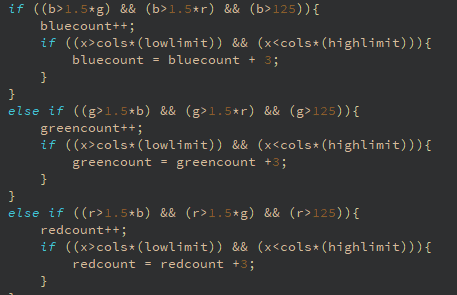
\includegraphics[width=2.5in]{t1}
\caption{Pixel testing code}
\label{fig_t1code}
\end{figure}

The code in figure \ref{fig_t1code} performs the checks needed to ascertain a pixel's primary colour. Initial attempts simply checked which of three component values were highest. In practice, this method was inaccurate as it had no way to differentiate between a near-white cell (such as a background cloud) which would have near equal \textit{RGB} values, and one that belonged to the subject (in this case, the car).

To allow the algorithm to differentiate between background elements and the subject, two methods were employed. Firstly, a pixel was only counted if that colour's value was a significant margin higher than the other values. In figure \ref{fig_t1code} this margin is $50\%$. Additionally, the pixel's value must be greater than half the colour space's maximum value, in this case, 125. This prevents background objects from being counted.


Additionally, extra weighting is applied to pixels within a central rectangular region of interest on the screen. This area can be changed by editing the values $highlimit$ and $lowlimit$. By adding this additional weighting to central areas, background areas are further discounted, helping to prevent false positives by valuing true positives more.

With the provided testing dataset of thirty red, blue, or green, cars this solution is 100$\%$ accurate, correctly identifying the subject's colour in every image. This is a marked improvement from the simple method used in the initial attempt, which would often get confused at reflections in windows (these would be reflecting the sky, which would add bias towards blue), background walls (especially brick, which would bias the results towards red), and any natural backgrounds (adding green bias).

An additional dataset was sourced of ninety images, thirty of each colour, to demonstrate the improvements' performance further. The results of this testing are visible in table \ref{testing_results1}.

\begin{table}[H]
% increase table row spacing, adjust to taste
%\renewcommand{\arraystretch}{1.3}
% if using array.sty, it might be a good idea to tweak the value of
% \extrarowheight as needed to properly center the text within the cells
\caption{Expanded dataset testing results}
\label{testing_results1}
\centering
\begin{tabular}{|c||c|}
\hline
Colour & Result\\
\hline
Red & 30/30\\
\hline
Green & 28/30\\
\hline
Blue & 30/30\\
\hline
\end{tabular}
\end{table}

For an overview of the algorithm's operation, see figure \ref{fig:task2_flowchart}.


\subsection{Limitations}
This solution is extremely limited in its current format. The solution has no form of object recognition, meaning that it cannot differentiate between the car that it is trying to find the colour of and any other objects inside the image. The middle-area weighting attempts to control for this; however, it assumes that the subject of the image is centre-frame, which cannot be said for all images of cars. This solution also has no way to deal with multiple cars in one image, especially ones of different colours. 

Additionally, using \textit{RGB} values is extremely limiting for colour recognition. The algorithm could not be expanded to detect additional colours (such as secondary colours made of a combination of red, green, and blue) without introducing a large amount of error. A major disadvantage of \textit{RGB} values is that they can vary greatly based on the lighting conditions present in the image. Other colour spaces isolate the brightness (or luma) value, allowing for changes in lighting to be compensated for. A further problem with \textit{RGB}'s representation of colour is that the hue is described as a combination of all three values, making it hard to isolate specific colours, as it is infrequent for any physical colour to exist in purely one colour channel.

\begin{figure}[h!]
\centering
\begin{subfigure}{0.225\textwidth}
    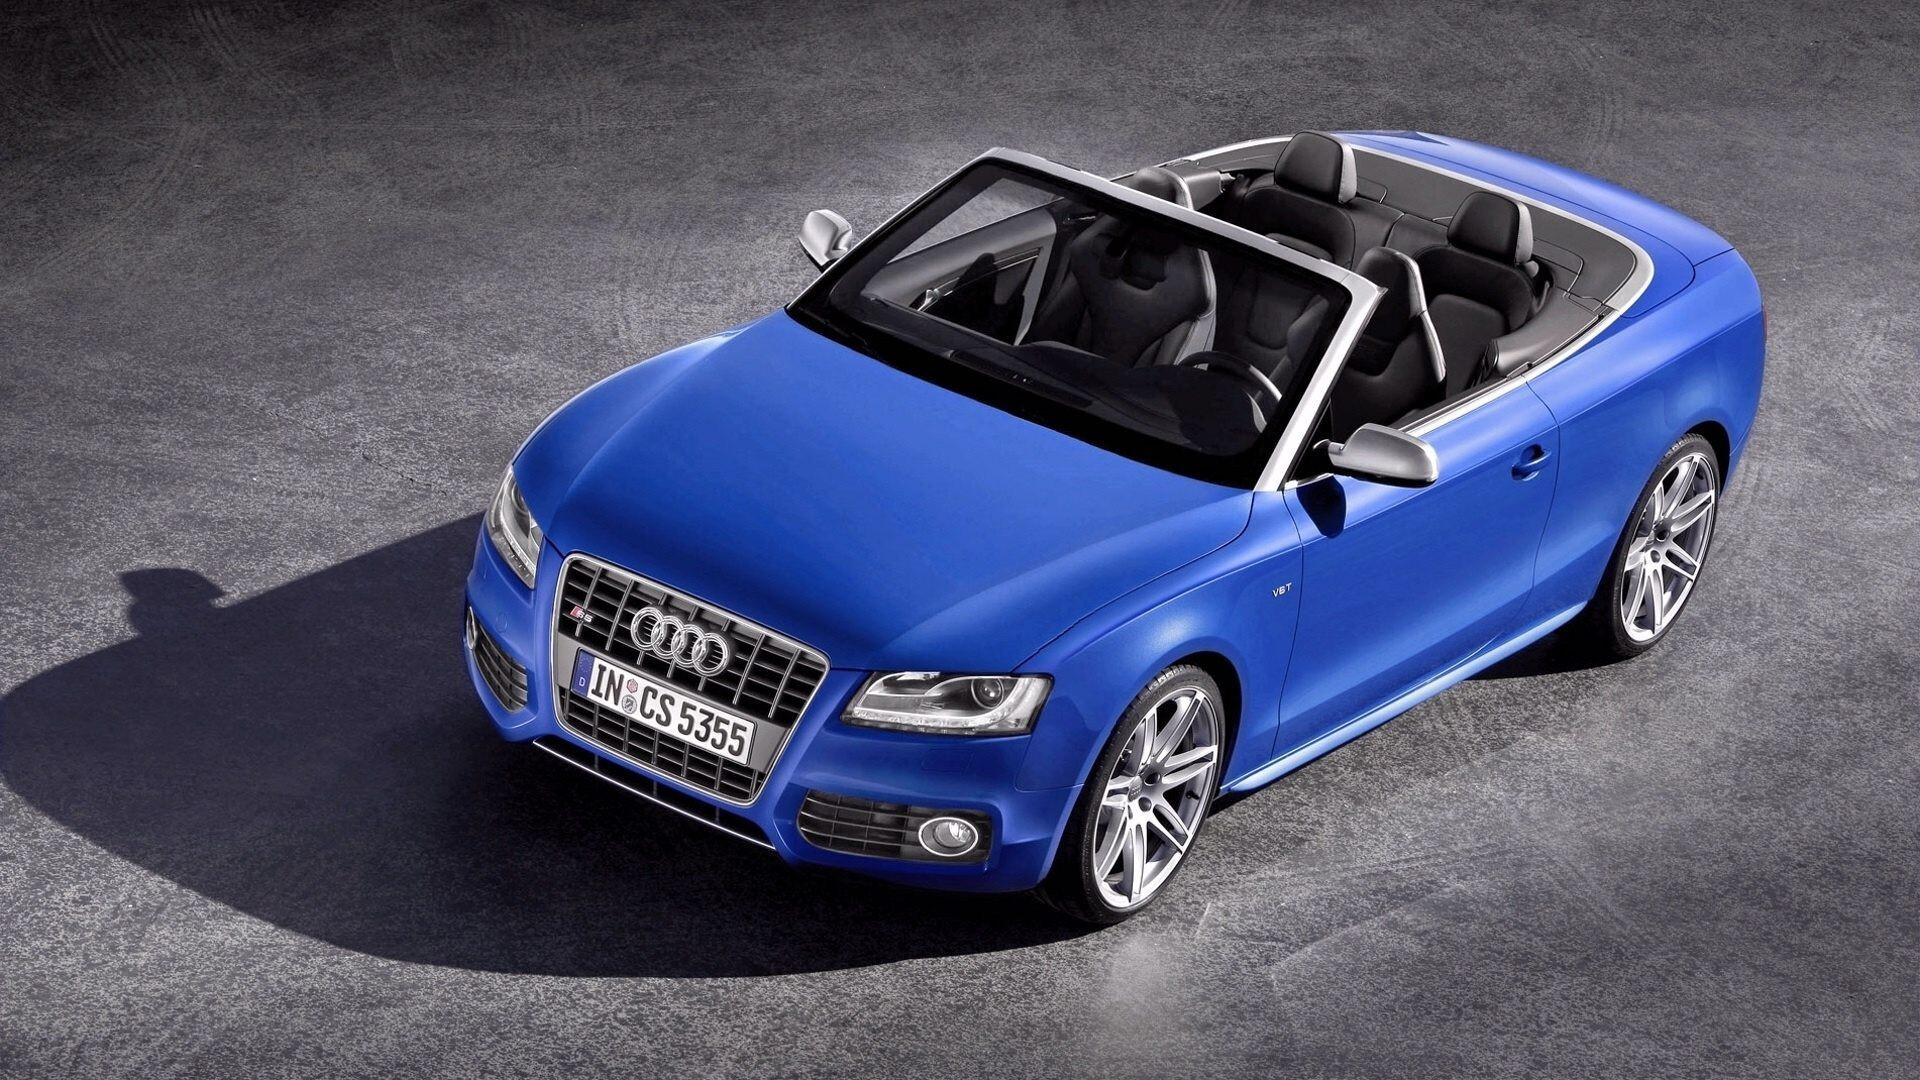
\includegraphics[width=\textwidth]{6}
    \caption{Image 6 (Green)}
    \label{fig:first}
\end{subfigure}
\hfill
\begin{subfigure}{0.225\textwidth}
    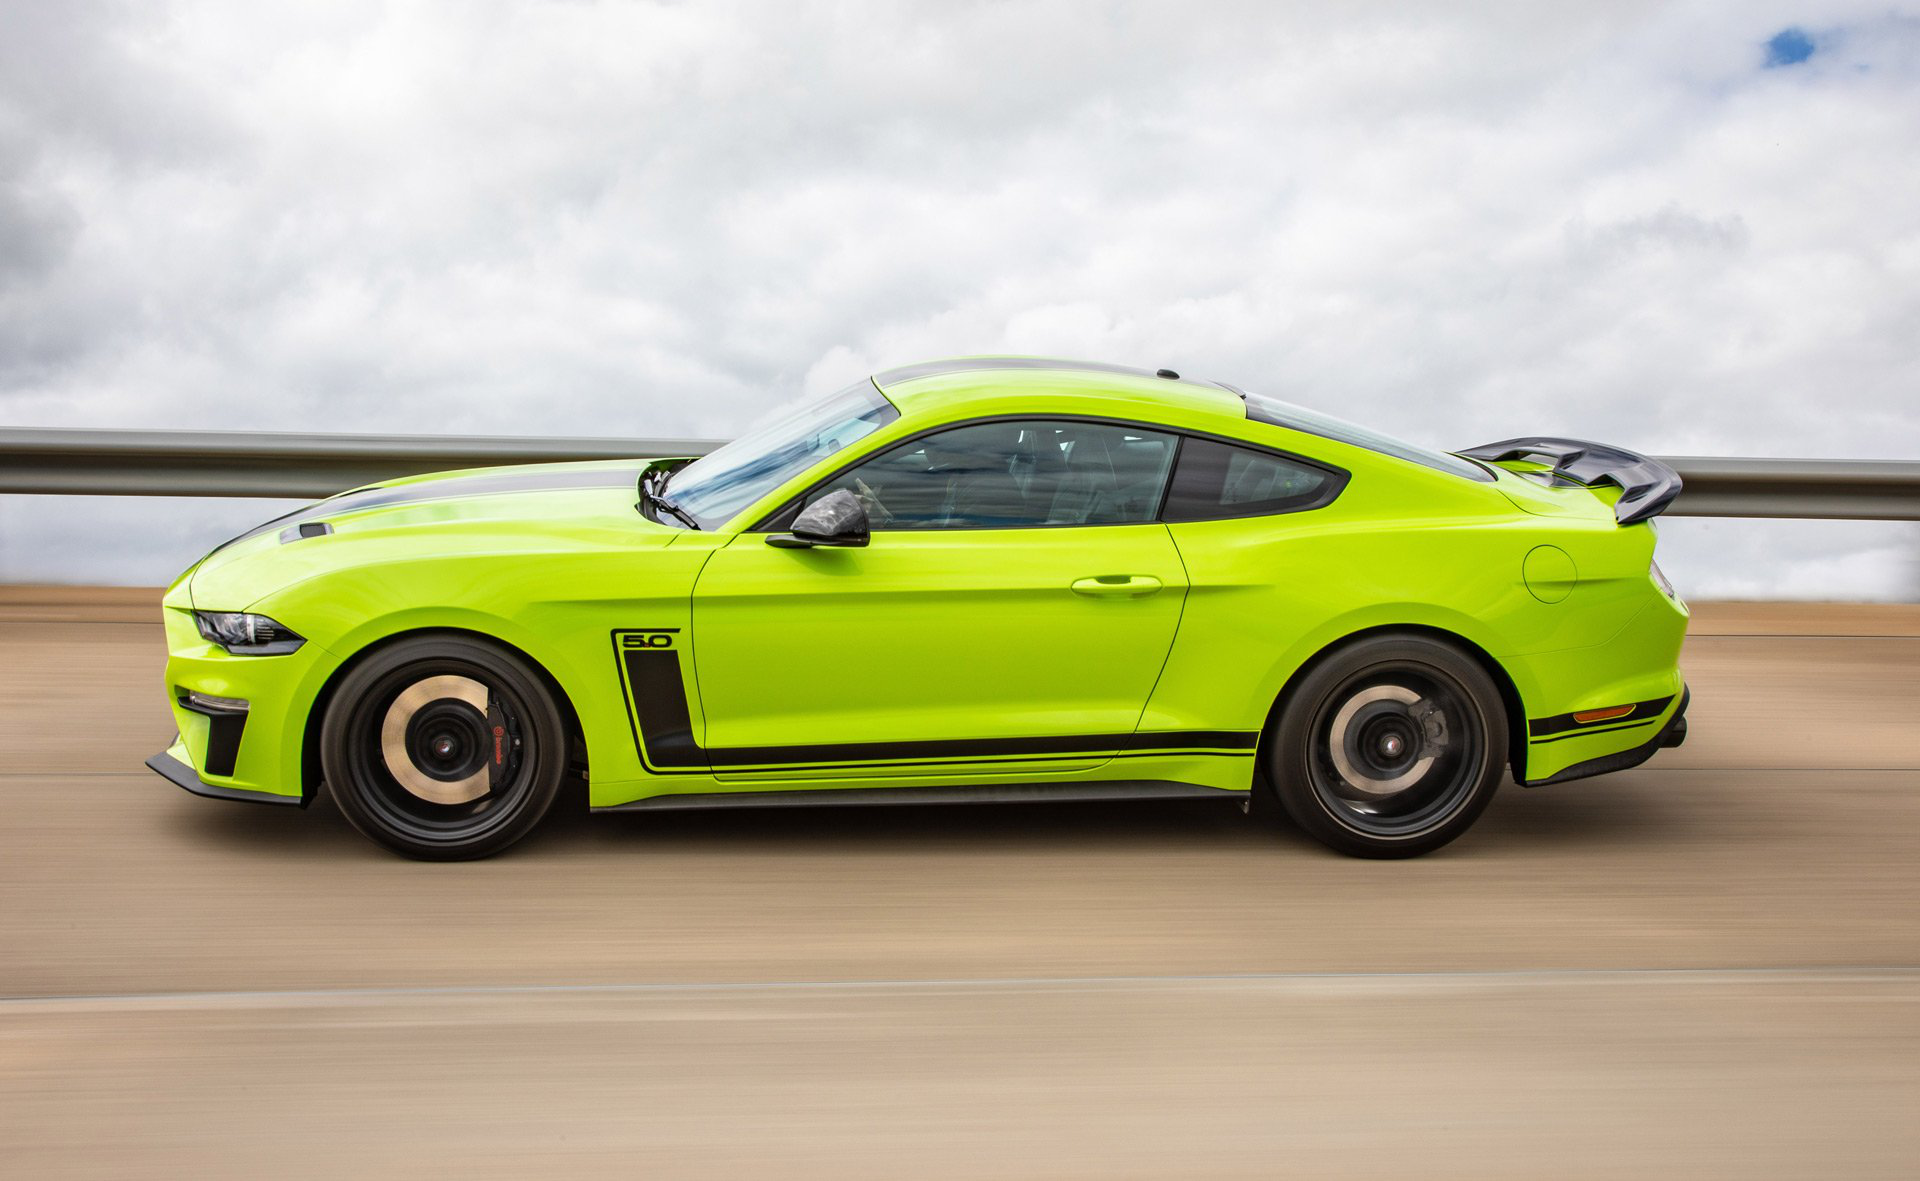
\includegraphics[width=\textwidth]{25}
    \caption{Image 25 (Green)}
    \label{fig:second}
\end{subfigure}

\begin{subfigure}{0.225\textwidth}
    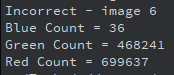
\includegraphics[width=\textwidth]{6_stats}
    \caption{Image 6 pixel count}
    \label{fig:third}
\end{subfigure}
\hfill
\begin{subfigure}{0.225\textwidth}
    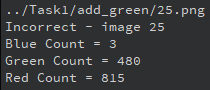
\includegraphics[width=\textwidth]{25_stats}
    \caption{Image 25 pixel count}
    \label{fig:fourth}
\end{subfigure}

\caption{Failed recognition images and stats}
\label{fig:fails}
\end{figure}

Figures \ref{fig:first} and \ref{fig:second} show images within the expanded dataset that the algorithm failed to categorise correctly, and their respective pixel counts in \subref{fig:third} and \subref{fig:fourth}. These images were both categorised as red despite the improvements made listed above. This is due to the large amounts of red coloured background elements (the reflection of the brake lights in \subref{fig:first} and the road surface in \subref{fig:second}).


\subsection{Further Improvements} \label{sec:further1}
A major improvement that could be made is switching colour space to \textit{HSV} instead of \textit{RGB}. \textit{HSV} has numerous benefits for colour recognition compared to \textit{RGB}, which are further elaborated on in section \ref{2_solution}.

Additionally, changing to \textit{HSV} would allow more colours to be recognised, as only the colour's \textit{hue} value would need to be programmed in for the algorithm to recognise it. This would allow for theoretically any colour to be recognised. Compared to \textit{RGB}, where each colour is a mixture of all three channels, this is much simpler to implement.

Colour recognition is possible within the \textit{RGB} colour space, however for enhanced accuracy a neural network could be employed\cite{inproceedings}. The specific implementation of the neural network would have it's own limitations, however, one common one would be a large amount of data would be required to correctly train the network. The dataset would need a much larger selection of images than the $120$ used in this implementation. 
\subsection{Conclusion}
This solution is adequate when the dataset is tightly controlled and consists only of red, green, or blue cars, with colour-neutral lighting in centre frame. Due to the limitations of both the approach and colour space, anything more than marginal performance increases would require significant changes to the methodology. Changing colour space to \textit{HSV} would provide a large increase in accuracy and allow for the solution to be expanded to cover more colours.

\section{Task 2 - Object Tracking}
\textit{For accompanying large figures, see appendix \ref{app:T2}}

\textit{For the video demo, click \href{https://youtu.be/kW5fbNTTovo}{HERE}}

The second task involves tracking a pendulum and using the observed displacement to calculate the pendulum's angular deviation from its vertical rest position.
\subsection{Introduction}
In order for the angle to be calculated, the pendulum's motion must be tracked. Fortunately, the pendulum arm has a green target affixed to the end. By isolating this colour from the background and calculating the centre of mass (CoM) using OpenCV's \textit{moments} functionality, the angle can be calculated using trigonometry.
\subsection{Solution}\label{2_solution}
The first stage of the solution is to find all the pixels that match the colour of the target on the pendulum arm. To do this, the colour space is first converted to \textit{HSV, \textbf{H}ue, \textbf{S}aturation, \textbf{V}alue.} \textit{HSV} has numerous benefits over \textit{RGB} for colour recognition\cite{RBGvHSV}, primarily that colours can easily be isolated using the \textit{hue} value, unlike in \textit{RGB}, where a colour is dependant on the values of all three channels.

 \textit{HSV} uses three values to describe a colour: \textit{hue}, \textit{saturation}, and \textit{value}. Light changes will only affect two of these values; the \textit{hue} value remains constant. This is better suited for colour recognition applications as it means changes in lighting, as well as natural minor differences in colours, can be compensated for with much tighter ranges than in any other colour space.

To isolate the target, \textit{OpenCV}'s \textit{inRange} function is used. This function takes four arguments, an input matrix, a vector of lower bounds, a vector of upper bounds, then an output matrix. The output matrix is monochrome, highlighting areas within the provided bounds in white and any that do not fall within these bounds in black. See appendix \ref{app:T2} to see the output of the program.

\begin{table}[H]
% increase table row spacing, adjust to taste
%\renewcommand{\arraystretch}{1.3}
% if using array.sty, it might be a good idea to tweak the value of
% \extrarowheight as needed to properly center the text within the cells
\caption{\textit{HSV} thresholds used inside the \textit{inRange} function}
\label{tab:t2thresholds}
\centering
\begin{tabular}{|c||c|c|}
\hline
Property & Lower Threshold & Upper Threshold\\
\hline
Hue & 70 & 80\\
\hline
Saturation & 30 & 255\\
\hline
Value & 30 & 255\\
\hline
\end{tabular}
\end{table}

As shown by table \ref{tab:t2thresholds}, the \textit{saturation} and \textit{value} variables have an extremely wide range to them, while still maintaining high accuracy. The narrow \textit{hue} range isolates the specific shade of green used on the target.

The centre of mass is calculated using the \textit{moments} function, then displayed as a point. To further aid the user, a cross hair is drawn over the centre of the target, with a line connecting it to the fulcrum at the top of the pendulum arm. For reference, an additional vertical line is drawn, representing an approximation of the vertical rest position.

The current angle is calculated by taking the arctangent, or inverse tangent, of the pendulum line.

\begin{equation}
angle = arctan(pendulum) - \frac{\pi}{4}
\end{equation}
An offset of $\pi /4$ is added to centre the graph around the 0 mark. Additionally, the angle is also displayed in degrees.

\begin{equation}
angle = x*(180/\pi )
\end{equation}

The calculated angle was written to a CSV file, figure \ref{fig:csv} which was then used to produce a graph, seen in figure \ref{fig_t2graph} within appendix \ref{app:T2}. Comparing the output graph to the observed behaviour of the systems shows that the results are as expected, with the pendulum acting equivalently to a dampened system returning to its rest state after receiving a stimulus.

\subsection{Limitations}\label{sec:t2_lim}
This implementation of object tracking does have its limitations. Firstly, it relies on the tracked target being a known colour, and also no other objects of a similar colour being observed by the input. This could be improved by using an additional technique to identify the target, for example, looking for a unique shape using edge detection or making the target more complex than a single colour, such as two colours in a tiled pattern.

Ideally, if visual detection is to be used, the target must be as unique as possible, to reduce the chances of objects within the camera's line of sight having enough similarity to confuse it. The current implementation relies on no objects being a similar shade of green, which works for the current scenario, but may be unreliable for less controlled applications. 

An additional issue with the optical based measurement employed here is that it relies on the target swinging on a path orthogonal to the camera. As shown in the output graph, there is a bias towards the positive direction, caused by the testing apparatus being slightly offset from the camera, distorting the results. This could be compensated for in software; however, it would be complex to implement, and such a solution's reliability cannot be speculated on.
\subsection{Further Improvements}
As discussed in section \ref{sec:t2_lim}, suggested improvements revolve around reducing the chance for non-target objects that have similar properties. This would involve increasing the relative complexity of the targets. For ease of implementation, the targets should have as many orders of rotational symmetry as possible to avoid having issues with having to recognise every rotational permutation of the target. \textit{OpenCV} provides documentation on recognising rotated images\cite{OpenCV_Rotate}. Additionally, a neural network could be trained to recognise the targets in any orientation or offset quickly enough to perform in real-time\cite{google}. An easy way to increase the complexity would be to add an additional distinctive colour and then have the software look for the two colours adjacent.

A Kalman filter could be implemented to improve the tracking performance\cite{Kalman}. The filter works by using the previous measurements and observations to estimate the state of this system, in this case, the pendulum's deviation. This would be helpful for any case where the video may not be as high quality, or the target may not be as clear.

While potentially outside the scope of the task, a generalised method for compensating for offset apparatus would increase the validity of the results, and help make any tests performed with this system more repeatable. Software based algorithms can perform this function with minimal latency \cite{5138693}. 
\subsection{Conclusion}
As per task one, this solution works extremely well in the controlled environment present in the video. However, increased robustness would be needed - provided either by an increase in target complexity, or additional tracking methods - to succeed in a less controlled environment.
\section{Task 3 - Cross Correlation}
\textit{For accompanying large figures, see appendix \ref{app:T3}}

\textit{For the video demo, click \href{https://youtu.be/Cwiae5Vpxyg}{HERE}}

The third task involves using cross-correlation to identify if components are present on a PCB.
\subsection{Introduction}
Cross-correlation in signal processing is used to measure the similarity between two signals, with the result being a function of displacement of the first signal relative to the second. The higher the result, the more closely related the two series are, with a perfect match meaning the two signals are effectively equal\cite{ControlStation}. 

Cross Correlation has numerous applications in image processing, such as searching a large image for a known feature. By using the \textit{OpenCV} \textit{matchTemplate} function, the point on an image that has the highest correlation can be identified, effectively revealing the location of the desired feature. 
\subsection{Solution}
The solution uses Normalised Square Difference Matching, presented as the argument \textit{'SQDIFF$\_$NORMED'} in \textit{OpenCV}. Using this matching method, the area with the best match will be presented as a local minima\cite{LearningOpenCV}, the code in figure \ref{fig_t3code} shows \textit{matchloc} being assigned the coordinate value of \textit{minloc}, which is passed by address into the \textit{minMaxLoc} function call.


\textit{minMaxLoc} is a built-in \textit{OpenCV} function that finds the global minimum and maximum in an array, and their respective positions\cite{OpenCV_minMaxLoc}. The extracted coordinates are used to draw a rectangle around the position of the component, with the size extracted from the component's associated \textit{png} file.

\begin{multline}
R_{sq\_diff\_normed} = \\ \frac{\sum_{x',y'}^{}[T(x',y')-I(x+x',y+y')]^2}{\sqrt{\sum_{x',y'}^{}T(x',y')^2 \bullet\sum_{x',y'}^{}I(x+x',y+y')}}
\end{multline}\label{eq:sq_diff}

\begin{figure}[h!]
\centering
\begin{subfigure}{0.35\textwidth}
    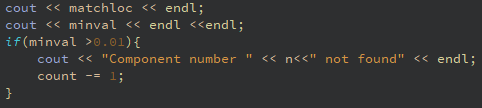
\includegraphics[width=\textwidth]{t3_code2}
    \caption{Error value check}
    \label{fig:t3_code2}
\end{subfigure}
\hfill
\begin{subfigure}{0.225\textwidth}
    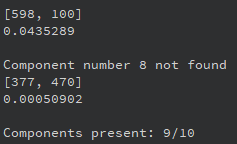
\includegraphics[width=\textwidth]{t3_outputTerminal}
    \caption{Terminal output showing missing component}
    \label{fig:t3_outputTerminal}
\end{subfigure}

\caption{Program response when a component is missing}
\label{fig:t3_output}
\end{figure}


%\begin{figure}[H]
%\centering
%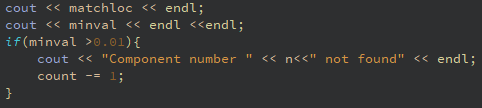
\includegraphics[width=2.5in]{t3_code2}
%\end{figure}   
%\begin{figure}[H]
%\centering
%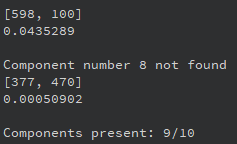
\includegraphics[width=2.5in]{t3_outputTerminal}
%\caption{a) Error value check \\b) associated terminal output.}
%\label{fig_t3code2}
%\end{figure}
The error threshold in figure \ref{fig:t3_code2} was chosen using experimentation. Inspection of the provided PCB image shows \textbf{U13} to be the missing component. This value was chosen by comparing the output values for present components with that of \textbf{U13} and selecting a threshold that would correctly isolate the missing component. 

\begin{table}[]
\caption{Error values of different components.}
\label{tab:t3error}
\begin{tabular}{|l|l|}
\hline
\textbf{Component} & \textbf{NMSD Error} \\ \hline
U4                 & 0.000642183         \\ \hline
C70                & 0.000428351         \\ \hline
U2                 & 0.000984659         \\ \hline
L2                 & 0.000689957         \\ \hline
Q1                 & 0.000671107         \\ \hline
C97                & 0.000465317         \\ \hline
C87                & 0.000600116         \\ \hline
U1                 & 0.00133448          \\ \hline
U13 (Missing)      & 0.0435289           \\ \hline
U13 (Present)      & 1.52745e-07         \\ \hline
L8                 & 0.00050902          \\ \hline
\end{tabular}
\end{table}

Table \ref{tab:t3error} shows the comparative error values between different components. It can be seen that the missing component, \textbf{U13}, has an error value an order of magnitude higher than the present components. To test the functionality of the solution, \textbf{U13} was edited back onto the board. The second iteration of the code performs the same checks against the complete board,and correctly identifies all components, reporting that all are found. Figure \ref{t3_outputTerminal2} shows the corresponding terminal output , while figure \ref{fig:t3_complete} within appendix \ref{app:T3} shows the results of the second execution.

\begin{figure}[H]
\centering
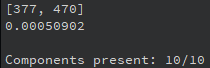
\includegraphics[width=2.5in]{t3_outputTerminal2}
\caption{Terminal output of the second execution, comparing against the complete board.}
\label{t3_outputTerminal2}
\end{figure}
\subsection{Limitations}
The major limitation of this implementation of template matching is that it does not account for differences in scale or orientation between the images to be matched. This means the images must match exactly; marginal differences in lighting or angle will cause greatly increased error values, potentially enough to cause an object not to be recognised. Whilst scale changes can be controlled for, any non-affine transformations (that is, transformations that do not preserve parallel lines) cannot be. 
\subsection{Further Improvements}
Differences in scale between the template image and the image to be searched can be rectified by performing the template match in a loop: the subject image is reduced in size slightly every iteration, until a match is found, or it is smaller than the template image. This can be augmented by performing edge map detections as opposed to just grey-scale representation, which would reduce issues with lighting changes, however would not help in the case of non-affine transformations\cite{MultiscaleDetection}.

In the case of non-affine transformations, such as distortions in the image, a better approach would be to use an alternative to template matching. One such alternative is to use Local Binary Patterns\cite{He1990TextureCU} to represent the features in the template and the image to be searched as Object Codes, comparing between the two \cite{Shen2013AFA}. This approach has better performance than standard template matching, and the use of SIFT(Scale Invariant Feature Transform)\cite{SIFT} and SURF (Speeded-Up Robust Features)\cite{BAY2008346} improves performance while allowing the algorithm to correctly identify the features regardless of any transforms applied to it.
\subsection{Conclusion}
This solution performs well in the controlled environment, with the template IC images being extracted directly from the source image. Under less than ideal conditions, this solution's performance would quickly drop off, as combinations of noise, image distortions, and changed lighting conditions would affect it. This could be improved by augmenting the template matching with edge map detection or using a more robust approach such as Object Codes.


% An example of a floating figure using the graphicx package.
% Note that \label must occur AFTER (or within) \caption.
% For figures, \caption should occur after the \includegraphics.
% Note that IEEEtran v1.7 and later has special internal code that
% is designed to preserve the operation of \label within \caption
% even when the captionsoff option is in effect. However, because
% of issues like this, it may be the safest practice to put all your
% \label just after \caption rather than within \caption{}.
%
% Reminder: the "draftcls" or "draftclsnofoot", not "draft", class
% option should be used if it is desired that the figures are to be
% displayed while in draft mode.
%
%\begin{figure}[H]
%\centering
%\includegraphics[width=2.5in]{myfigure}
% where an .eps filename suffix will be assumed under latex, 
% and a .pdf suffix will be assumed for pdflatex; or what has been declared
% via \DeclareGraphicsExtensions.
%\caption{Simulation Results}
%\label{fig_sim}
%\end{figure}

% Note that IEEE typically puts floats only at the top, even when this
% results in a large percentage of a column being occupied by floats.


% An example of a double column floating figure using two subfigures.
% (The subfig.sty package must be loaded for this to work.)
% The subfigure \label commands are set within each subfloat command, the
% \label for the overall figure must come after \caption.
% \hfil must be used as a separator to get equal spacing.
% The subfigure.sty package works much the same way, except \subfigure is
% used instead of \subfloat.
%
%\begin{figure*}[!t]
%\centerline{\subfloat[Case I]\includegraphics[width=2.5in]{subfigcase1}%
%\label{fig_first_case}}
%\hfil
%\subfloat[Case II]{\includegraphics[width=2.5in]{subfigcase2}%
%\label{fig_second_case}}}
%\caption{Simulation results}
%\label{fig_sim}
%\end{figure*}
%
% Note that often IEEE papers with subfigures do not employ subfigure
% captions (using the optional argument to \subfloat), but instead will
% reference/describe all of them (a), (b), etc., within the main caption.


% An example of a floating table. Note that, for IEEE style tables, the 
% \caption command should come BEFORE the table. Table text will default to
% \footnotesize as IEEE normally uses this smaller font for tables.
% The \label must come after \caption as always.
%
%\begin{table}[!t]
%% increase table row spacing, adjust to taste
%\renewcommand{\arraystretch}{1.3}
% if using array.sty, it might be a good idea to tweak the value of
% \extrarowheight as needed to properly center the text within the cells
%\caption{An Example of a Table}
%\label{table_example}
%\centering
%% Some packages, such as MDW tools, offer better commands for making tables
%% than the plain LaTeX2e tabular which is used here.
%\begin{tabular}{|c||c|}
%\hline
%One & Two\\
%\hline
%Three & Four\\
%\hline
%\end{tabular}
%\end{table}


% Note that IEEE does not put floats in the very first column - or typically
% anywhere on the first page for that matter. Also, in-text middle ("here")
% positioning is not used. Most IEEE journals/conferences use top floats
% exclusively. Note that, LaTeX2e, unlike IEEE journals/conferences, places
% footnotes above bottom floats. This can be corrected via the \fnbelowfloat
% command of the stfloats package.


\newpage
\appendix

\printbibliography


\onecolumn
\subsection{Github Repository}

For the full code, please see the linked github repository \href{https://github.com/jjpendlebury/AINT308-Coursework}{HERE}.
\subsection{Task 1 Figures}\label{app:T1}

\begin{figure}[H]
\centering
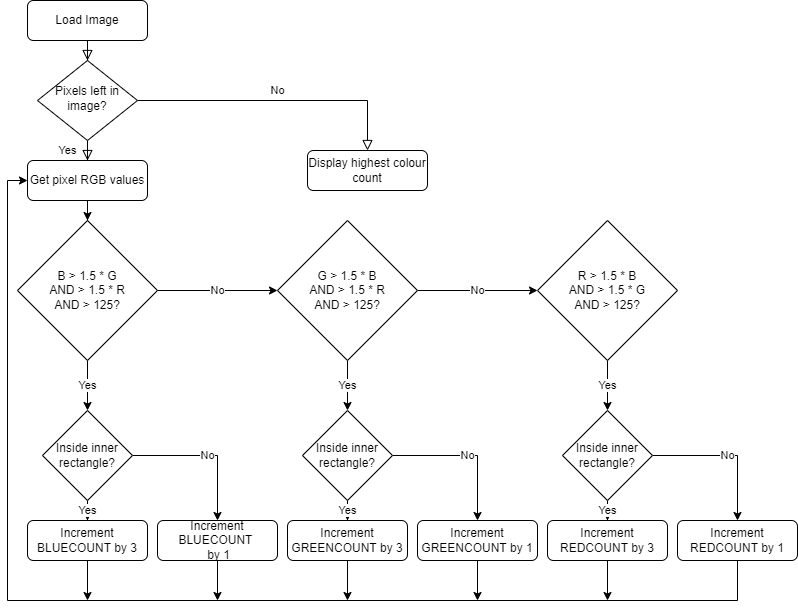
\includegraphics[width=5in]{Task1_flowchart}
\caption{Flowchart showing the Task 1 algorithm}
\label{fig:task1_flowchart}
\end{figure}

\subsection{Task 2 Figures}\label{app:T2}

\begin{figure}[H]
\centering
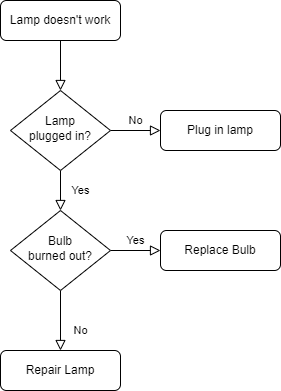
\includegraphics[width=4in]{Task2_flowchart}
\caption{Flowchart showing the Task 2 algorithm}
\label{fig:task2_flowchart}
\end{figure}

\begin{figure}[H]
\centering
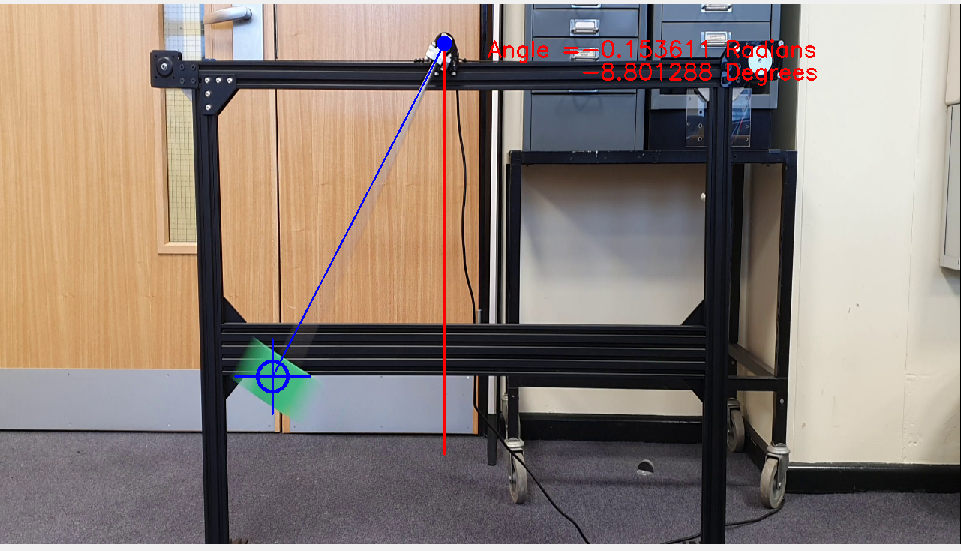
\includegraphics[width=5in]{t2_output2}
\end{figure}
\begin{figure}[H]
\centering
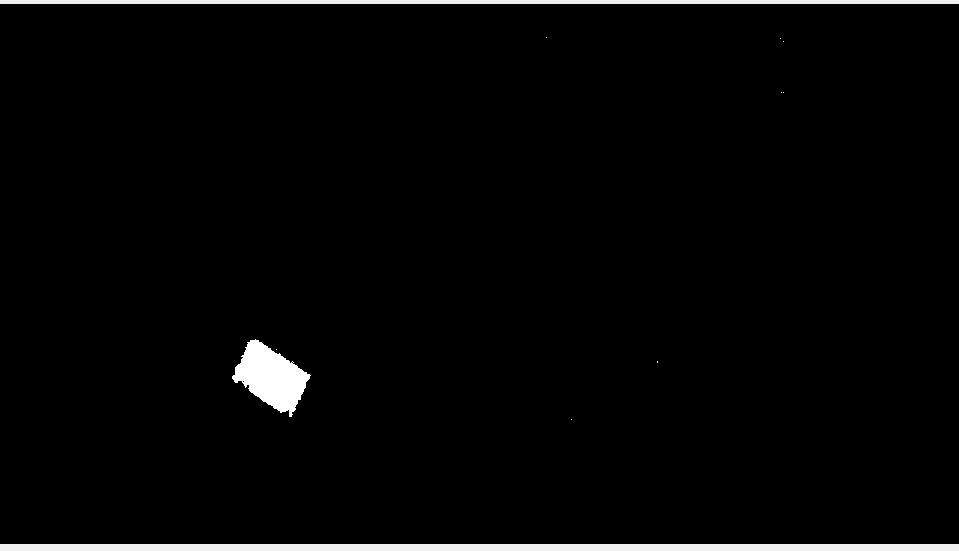
\includegraphics[width=5in]{t2_output3}
\caption{Single frame of output from Task 2's execution. Note the green target is highlighted in the second frame.}
\label{fig_t2output}
\end{figure}
\begin{figure}[H]
\centering
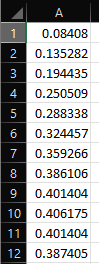
\includegraphics[width=1in]{csv}
\caption{Snippet of the CSV file that data is written to, showing the deviation measured in the first twelve frames of video.}
\label{fig:csv}
\end{figure}
\begin{figure}[H]
\centering
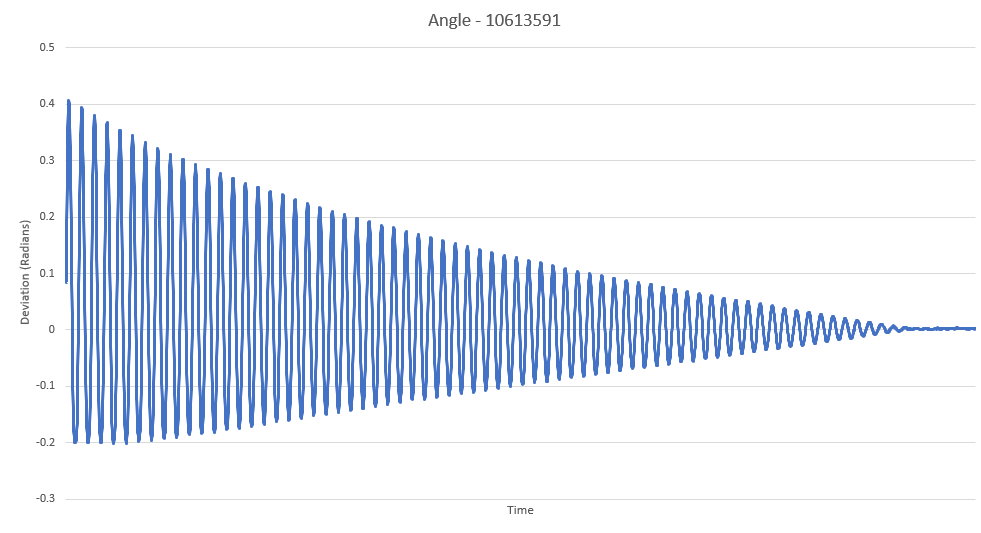
\includegraphics[width=5in]{t2_graph}
\caption{Output graph showing the pendulum's deviation from the vertical plotted against time. The raw data and graph is available for edit within the archive.}
\label{fig_t2graph}
\end{figure}


\subsection{Task 3 Figures}\label{app:T3}
\begin{figure}[H]
\centering
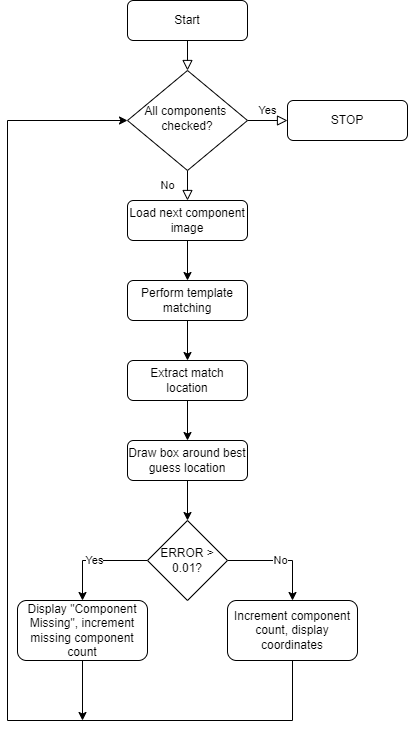
\includegraphics[width=4in]{Task3_flowchart}
\caption{Flowchart showing the Task 3 algorithm}
\label{fig:task2_flowchart}
\end{figure}

\begin{figure}[H]
\centering
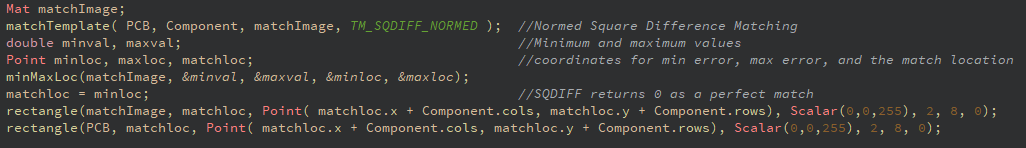
\includegraphics[width=5in]{t3_code1}
\caption{Template matching code, showing use of Normalised Squared Difference Matching.}
\label{fig_t3code}
\end{figure}

\begin{figure}[H]
\centering
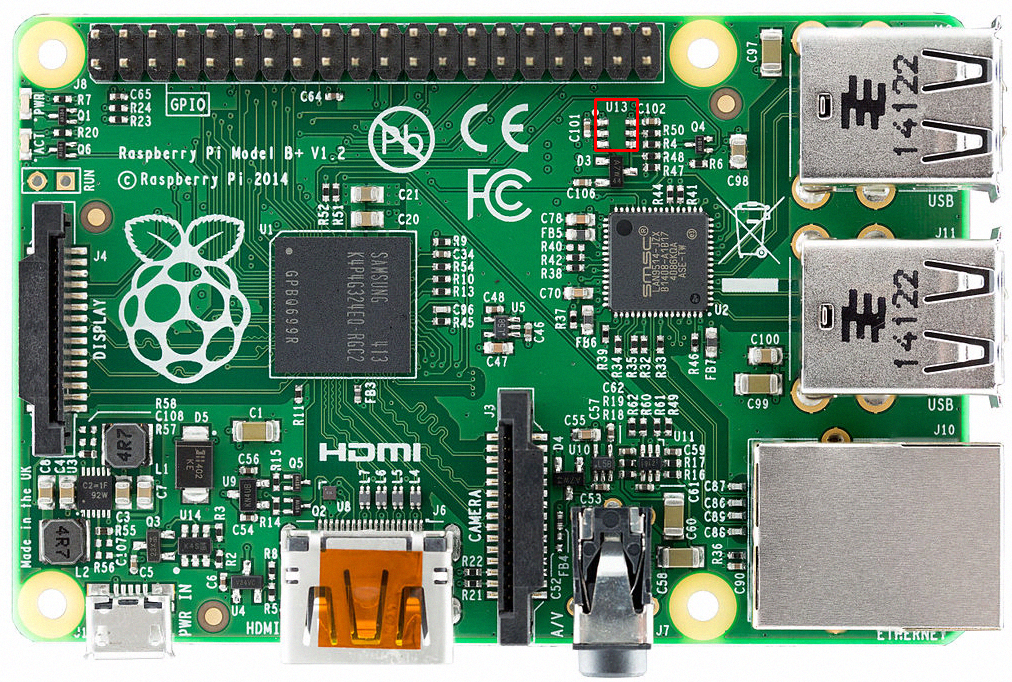
\includegraphics[width=5in]{t3_missing}
\caption{Task 3 output showing the position of \textbf{U13} correctly highlighted as the missing component.}
\label{fig:t3_missing}
\end{figure}
\begin{figure}[H]
\centering
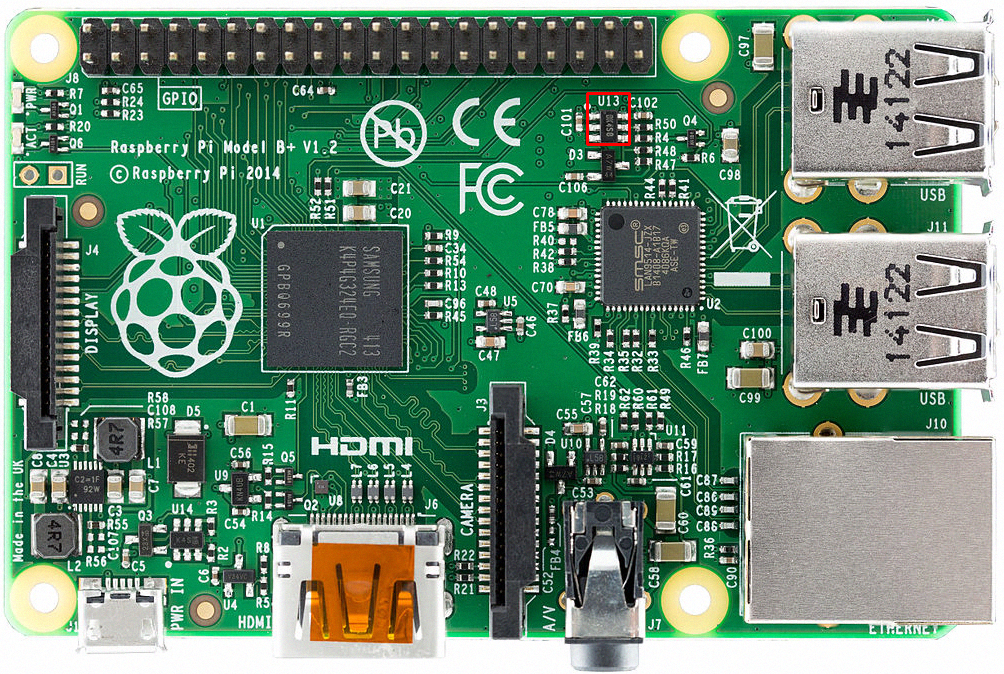
\includegraphics[width=5in]{t3_complete}
\caption{The edited PCB image with \textbf{U13} identified.}
\label{fig:t3_complete}
\end{figure}
\subsection{Code Printouts}
The following pages contain complete printouts of the code used to implement the solutions outlined above, for reference.
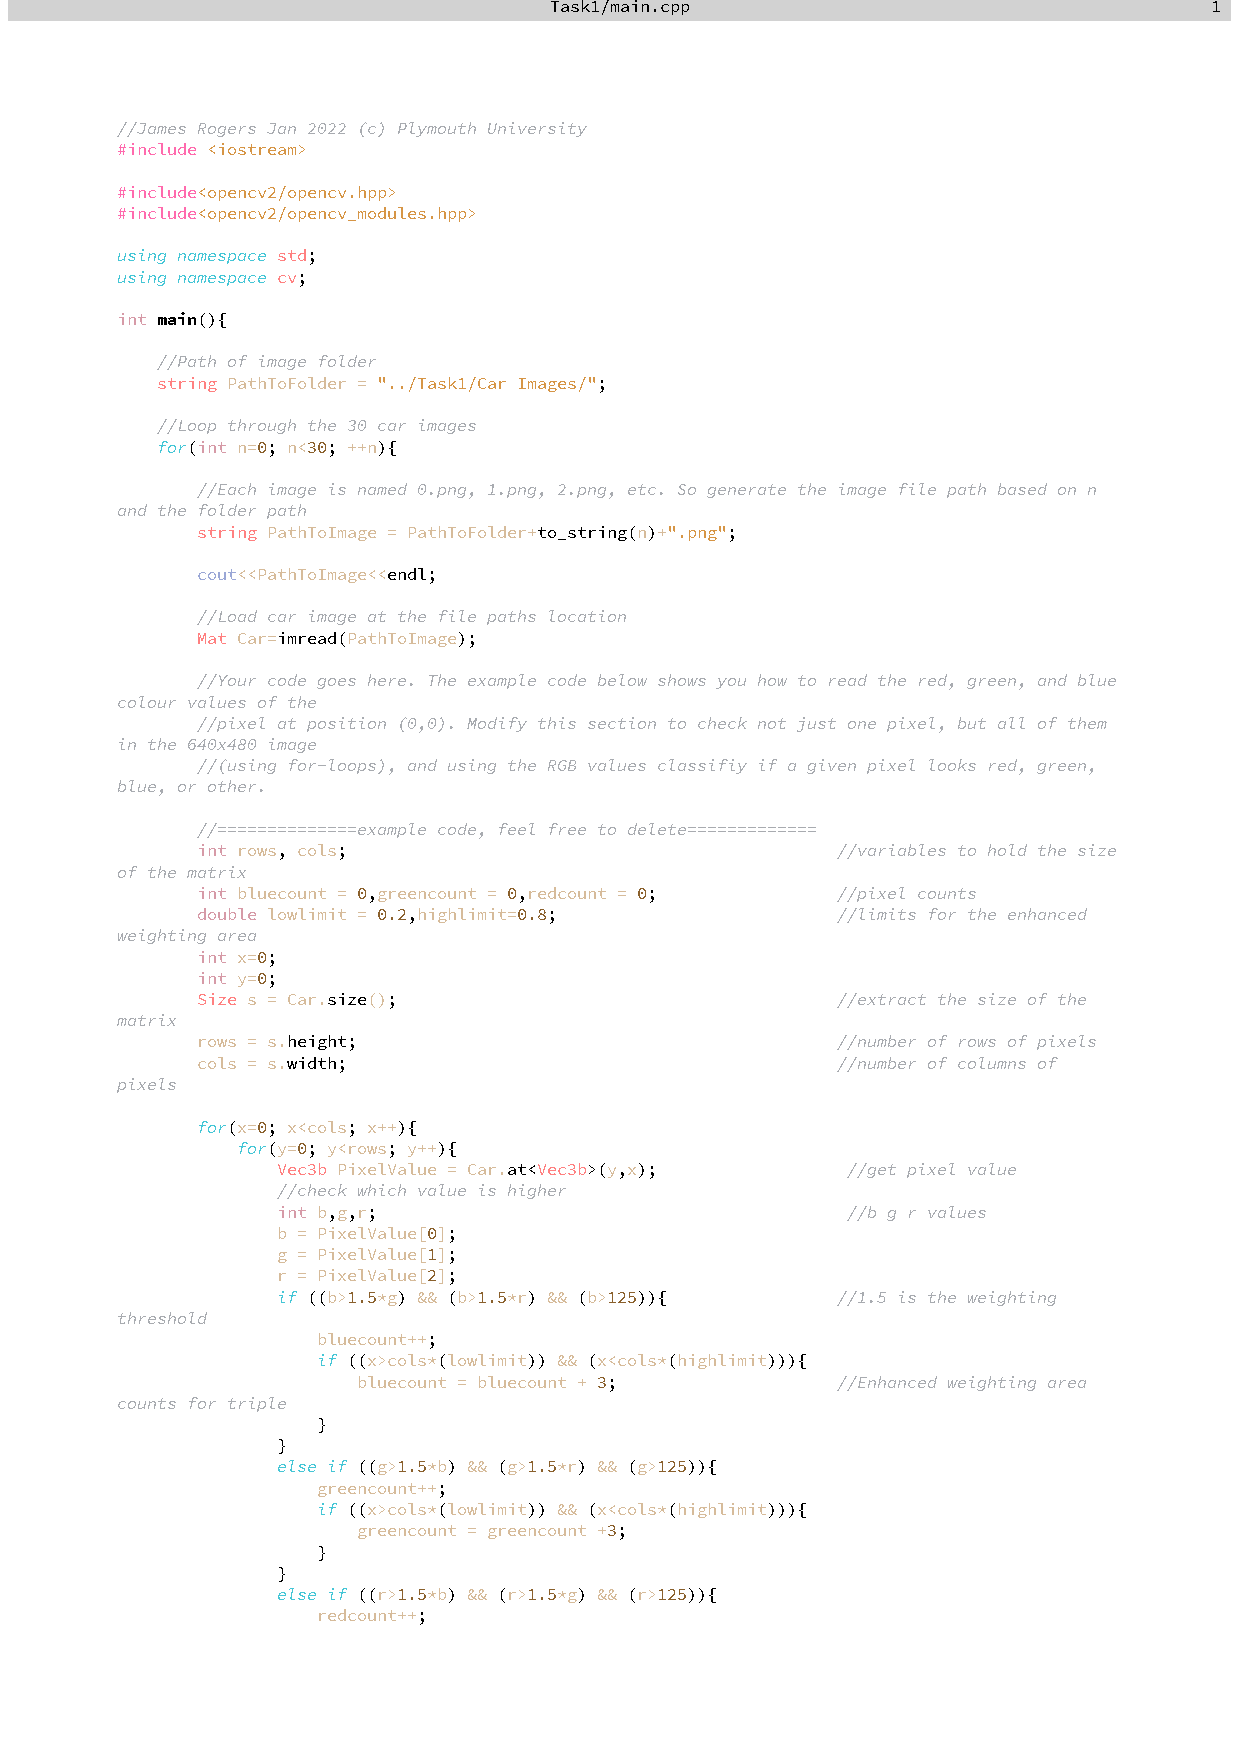
\includepdf[pages=-,offset=0 -50]{task1_code.pdf}
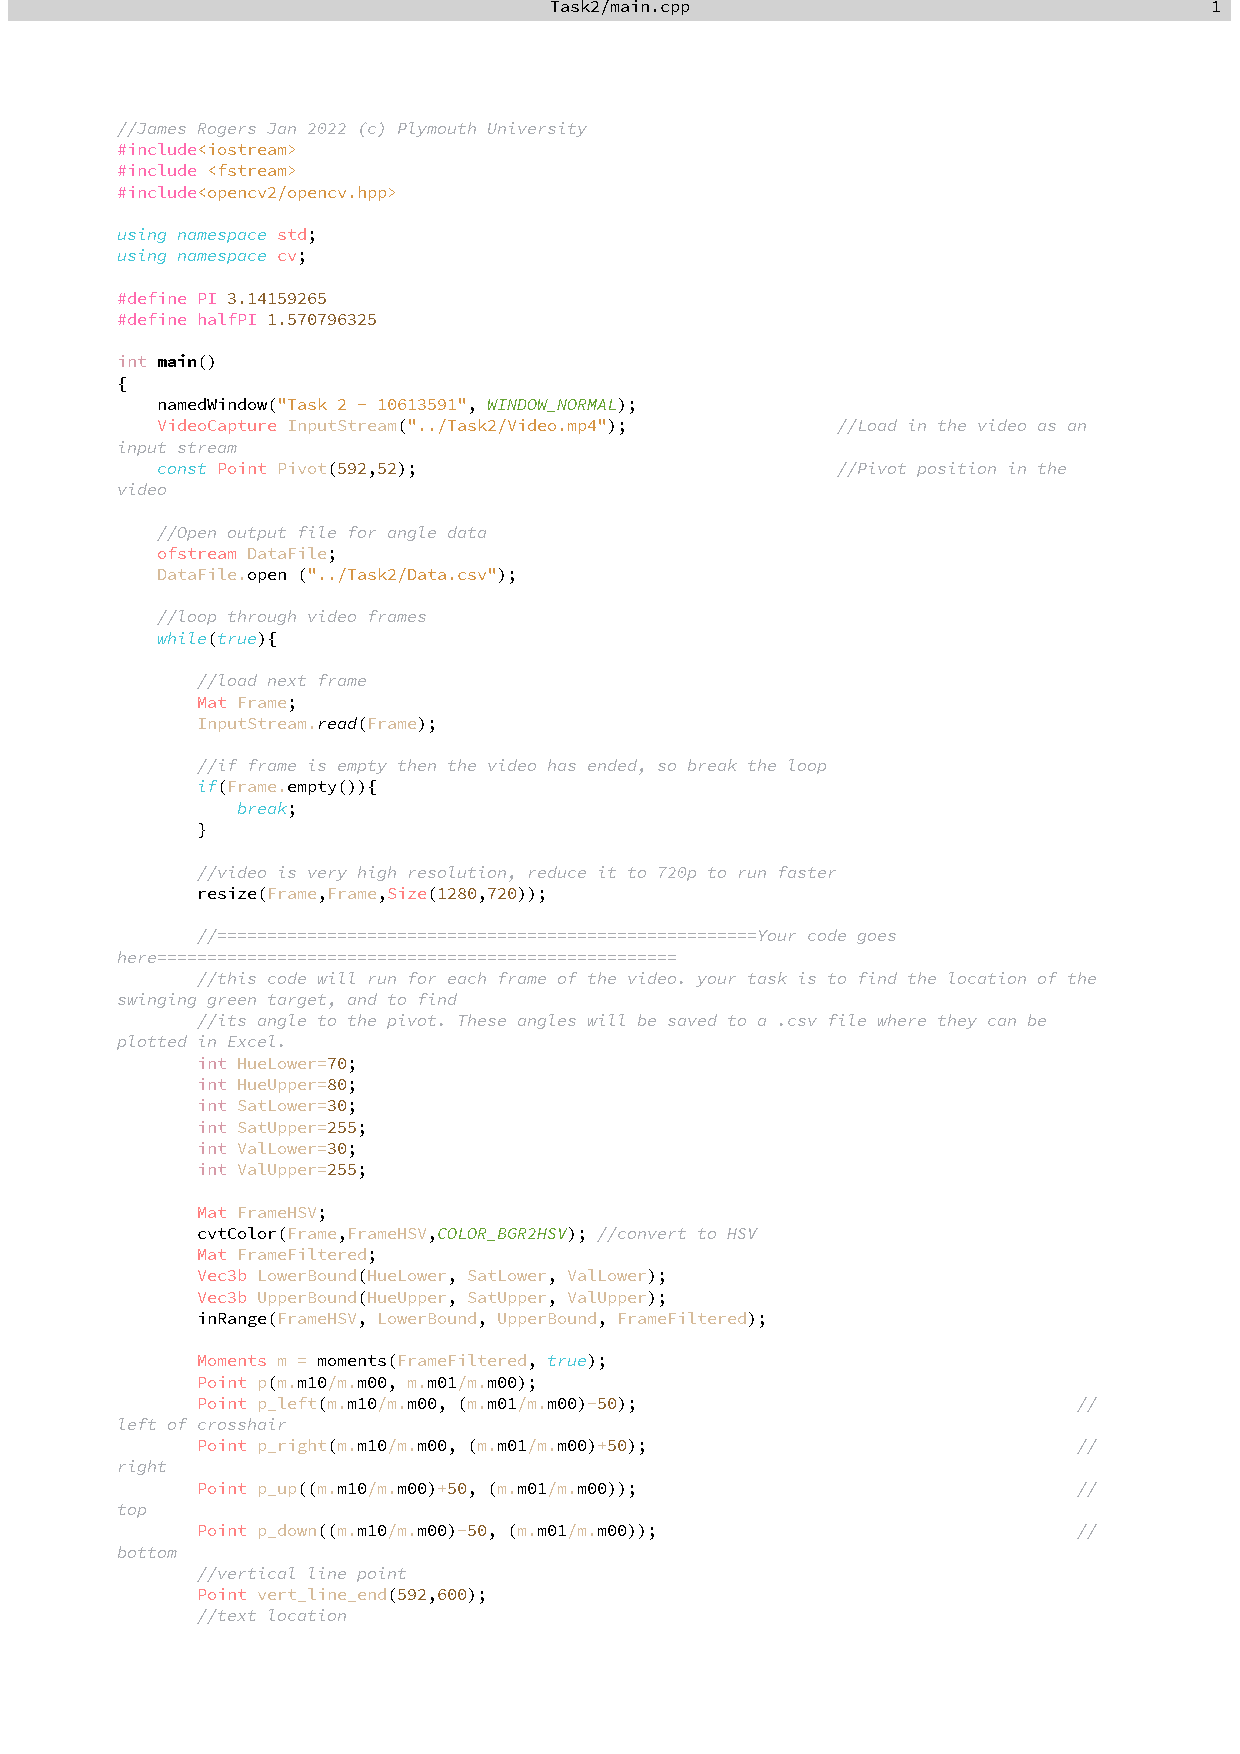
\includepdf[pages=-,offset=0 -50]{task2_code.pdf}
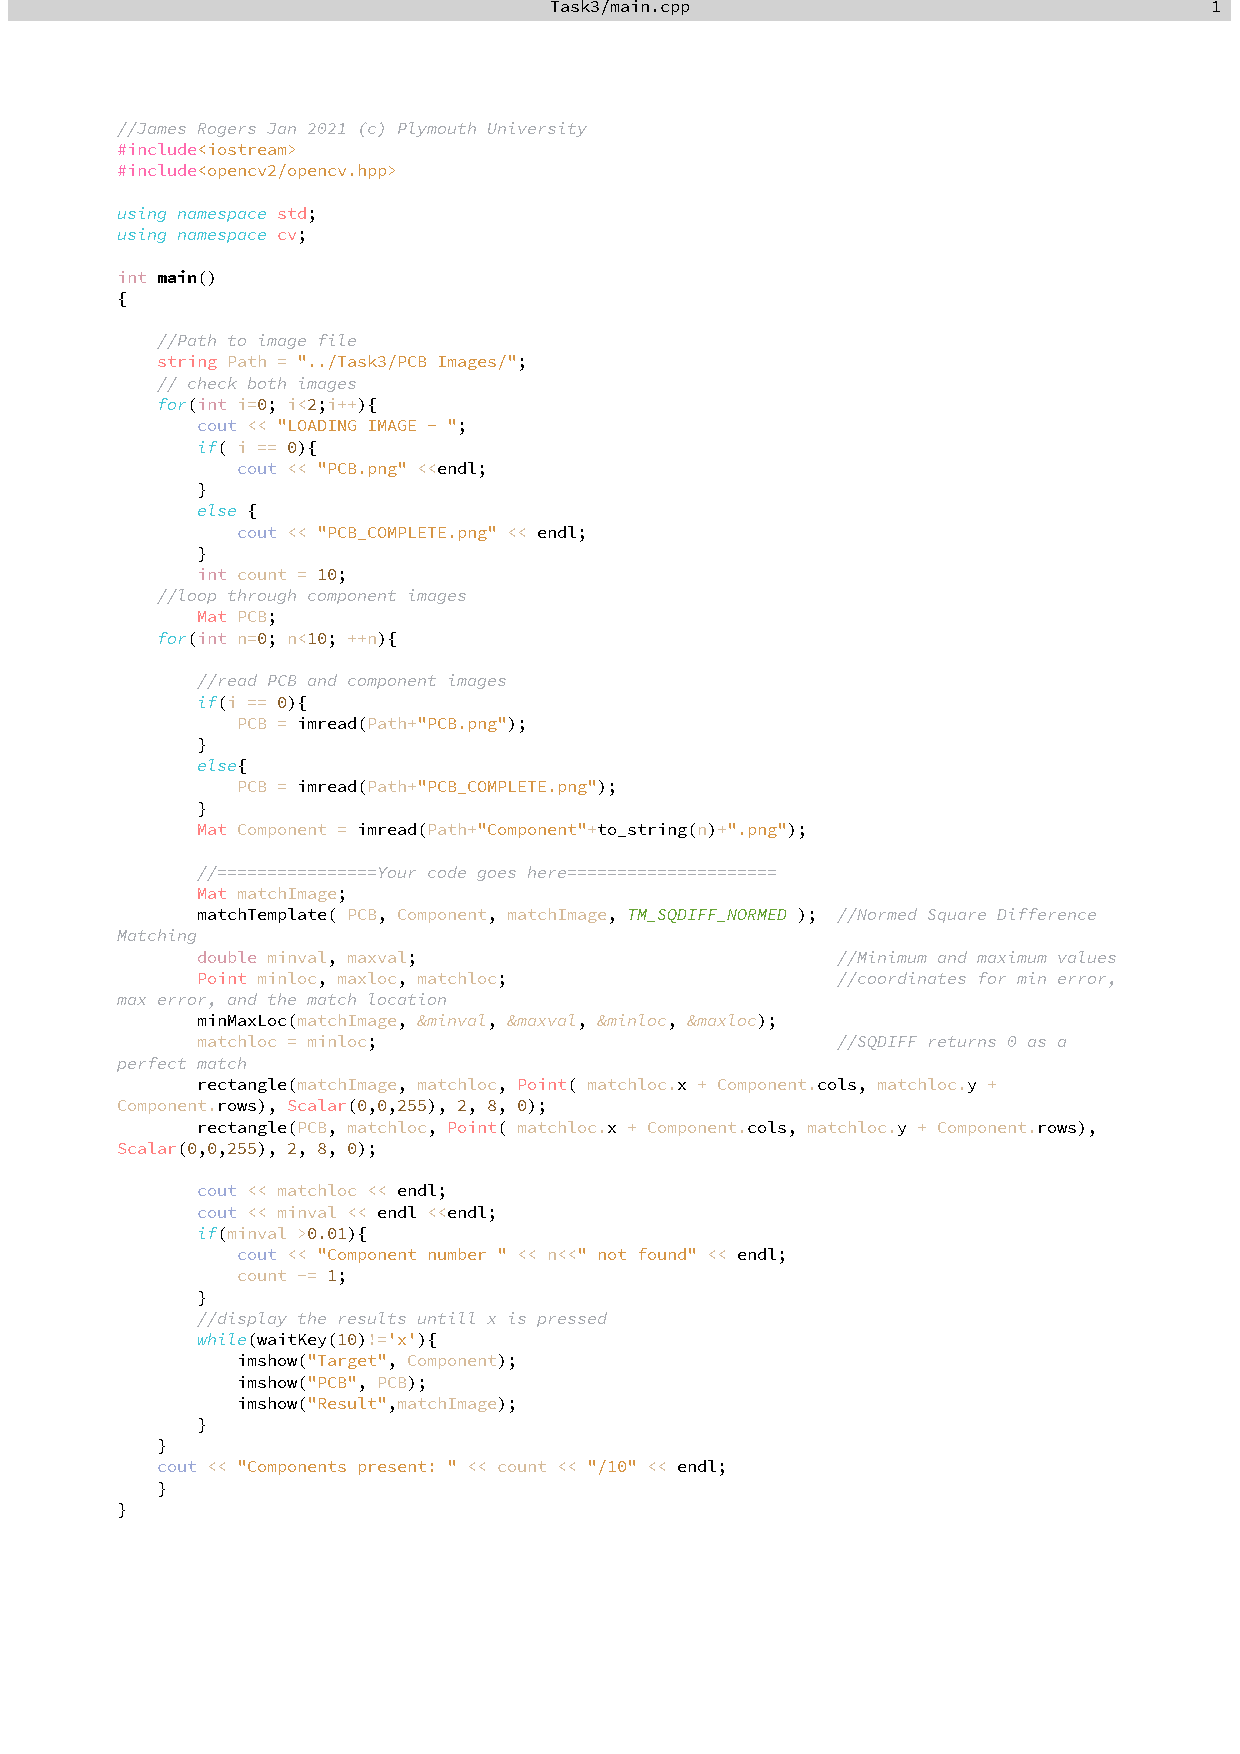
\includepdf[pages=-,offset=0 -50]{task3_code.pdf}
% that's all folks
\end{document}